\documentclass[a4j]{jarticle}
\usepackage[dvipdfmx]{graphicx}

\begin{document}
本稿では,1対1のシューティングを想定する.お互いの移動はランダムであり,撃つ側のプレイヤーは十分遠くから, 相手プレイヤーの中心を正確に狙って攻撃するものとする.また弾速は無限大とする.

\begin{figure}[tb]
\begin{center}
	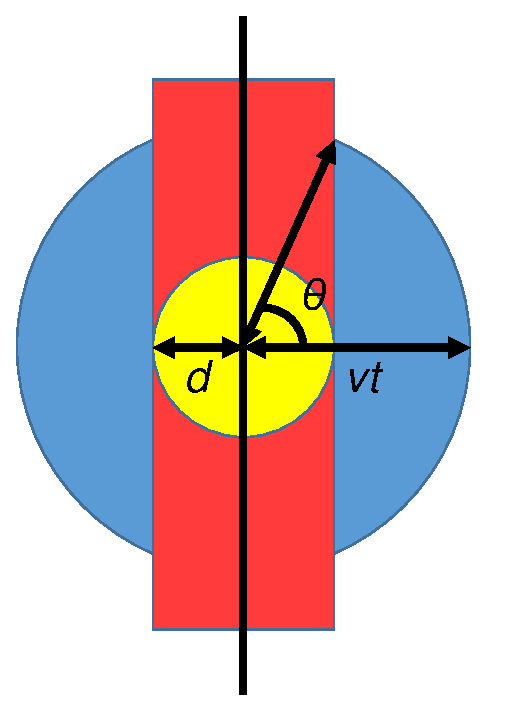
\includegraphics[width=5.0cm]{モデル図.eps}
	\caption{提案モデル}
\end{center}
\end{figure}

想定するモデルを図1に示す. 黄色の円はプレイヤーの当たり判定を,青い円がプレイヤーが移動しうる範囲を表している.弾丸が黒い線を通過する際,プレイヤーが赤い帯の内部に居る場合命中し,そうでない場合命中しない.またプレイヤーが存在する確率を一様とすると,弾丸の命中率は青い円の中で赤い帯が占める割合と一致する.この割合は,当たり判定の半径を$d$, 移動速度を$v$,遅延時間を$t$,$\cos \theta = d/v t$とすると, 
\begin{equation}
\frac{\pi(vt)^2(\frac{2\pi-4\theta}{2\pi})+2dvt\sin\theta}{\pi (vt)^2}
\end{equation}
と表せる.
よって,弾丸を一発撃った時,その弾丸が命中する確率は,  
\begin{equation}
1-\frac{2\theta}{\pi}+\frac{\sin2\theta}{2\pi}
\end{equation}
となる.

$d=0.5$(m), $v=5$(m/s)の条件下で$t$を変化させた場合の命中率を図2,3に示す.図3は図2の一部を拡大したものである.
\begin{figure}[b]
\begin{minipage}{0.5\hsize}
\begin{center}
	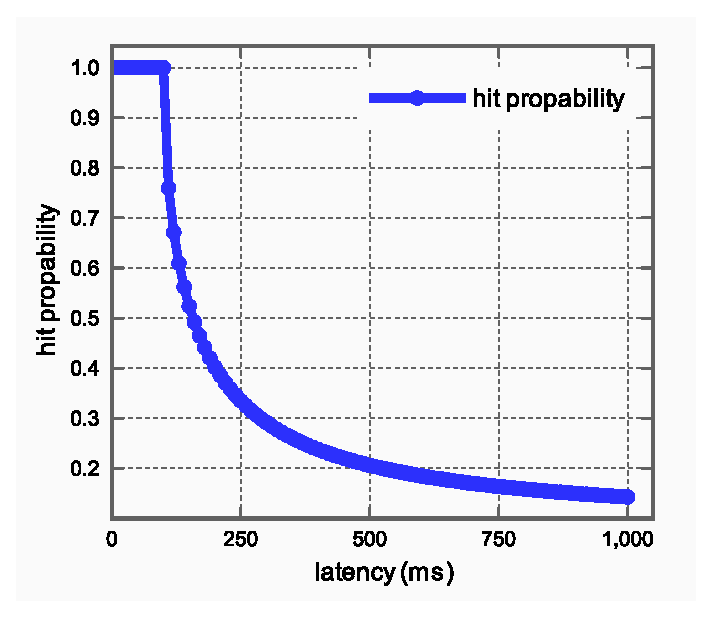
\includegraphics[width=5.0cm]{1000mstest.eps}
	\caption{結果}
\end{center}
\end{minipage}
\begin{minipage}{0.5\hsize}
\begin{center}
	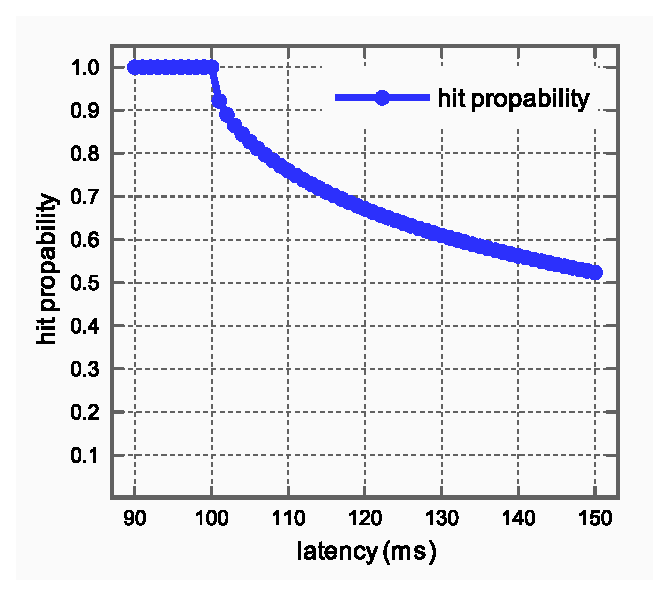
\includegraphics[width=5.0cm]{150mstest.eps}
	\caption{結果(拡大図)}
\end{center}
\end{minipage}
\end{figure}
\end{document}
